\chapter{Sample Imputation via Conditional Residual Denoising Diffusion Networks}
\label{chap:SIRD}

\section{Introduction}
\label{sec:sird_intro}

Chapter~\ref{chap:SISL} considered Design~I, where the outcome component of the joint sampling stratum is observed, the variables $S_1$ and $S_2$ are hidden, and the design weight is released. SISL uses that weight in a sample-likelihood correction. Chapter~\ref{chap:SICG} developed an adversarial generator for settings in which the observed phase-one block can identify the target conditional distribution. Both that method and the chained-equation comparators treat the phase-one proxy $\tilde X_i$ as one conditioning covariate among the others, which may not make full use of the information it carries. SIRD instead gives the paired proxy a more specific role. For a continuous measurement, it models the residual $\tilde X_i-X_i$ around the observed proxy. For a categorical measurement, the validated pairs estimate transitions from proxy category to validated category. These two roles define the diffusion paths developed below.

The diffusion imputation methods reviewed in Section~\ref{sec:diffusion} do not use the phase-one proxy in this way. CSDI \citep{tashiro2021csdi} and its tabular adaptation TabCSDI \citep{zheng2022diffusion} inherit the denoising diffusion probabilistic model (DDPM) construction of \citet{ho2020denoising}, in which the forward process corrupts the data toward Gaussian noise and the reverse process reconstructs the missing entries conditional on the observed entries. Two features of this construction are not tailored to the present validation designs. First, as discussed in Section~\ref{sec:3.5.4}, TabCSDI is trained by self-supervised random masking, although the missingness pattern in a two-phase validation study is fixed by \(R_i\) and known to the analyst. The extra masking is useful for a general imputation method that must handle many missingness patterns, but in this setting it consumes part of the already limited validated signal. Second, TabCSDI represents categorical variables through an encoded continuous state rather than through a transition law between the phase-one and phase-two categories. These choices are reasonable for a general-purpose diffusion model, but they do not use the paired proxy as the endpoint of the generative path.

Sample Imputation via Conditional Residual Denoising Diffusion Networks (SIRD) is developed to test this alternative use of the proxy. The continuous component borrows from residual diffusion for restoration: instead of forcing the forward chain to discard the record and then asking the reverse chain to rebuild it from noise, the chain is made to end near the observed degraded measurement. For paired continuous variables, this means moving the validated value \(X_i\) toward the observed proxy \(\tilde{X}_i\), so reverse sampling for an unvalidated individual begins from that individual's own phase-one measurement. For paired categorical variables, the phase-one partner supplies transition information rather than a numerical residual. The chapter also re-evaluates the parameter-uncertainty mechanisms studied for SICG, namely MC-dropout \citep{gal2016dropout}, bootstrap retraining, and SWAG \citep{maddox2019simple}, because their behaviour need not transfer from an adversarial generator to a diffusion denoiser.

Section~\ref{sec:sird_background} reviews the continuous and categorical diffusion choices that were not covered by the DDPM-based account in Section~\ref{sec:diffusion}. Section~\ref{sec:sird_method} gives the SIRD construction. Section~\ref{sec:sird_ablation} reports the ablation decisions, including the uncertainty-injection mechanism. Section~\ref{sec:sird_sim} reports the simulation results under the framework of Chapter~\ref{chap:SimDesigns}. Section~\ref{sec:sird_discussion} discusses the findings.


\section{Background}
\label{sec:sird_background}

The DDPM construction, the score-based perspective, and the conditional diffusion imputation methods CSDI and TabCSDI were described in Section~\ref{sec:diffusion}. The present section reviews the two parts of the diffusion literature that are needed for SIRD but were not central in that earlier review. The first is residual diffusion for continuous variables, where the forward process can terminate near an observed degraded measurement instead of an uninformative noise distribution. The second is diffusion on discrete categorical states, where the transition structure can encode prior information about likely category changes. These two ideas are needed together because the phase-two block in the thesis contains both continuous measurements and misclassified categorical variables.


\subsection{Continuous proxy-anchored diffusion}
\label{sec:sird_rddm}

In the DDPM forward process of equation~\eqref{eq:ddpm_forward}, the marginal corrupted state can be written as \(x_t = \sqrt{\bar{\alpha}_t}\,x_0 + \sqrt{1-\bar{\alpha}_t}\epsilon\), with \(\epsilon\sim\mathcal{N}(0,I)\) and \(\bar{\alpha}_t\) decreasing toward zero. As \(t\) approaches the end of the chain, the marginal state approaches isotropic Gaussian noise and no longer carries record-level information about \(x_0\). The reverse model must therefore learn a path from an uninformative endpoint back to the data distribution. This is a natural construction for unconditional generation. It is less direct for a validation study in which a degraded measurement of the same target quantity is already observed for every unit.

Residual Denoising Diffusion Models (RDDM) were introduced for restoration tasks in which such a degraded reference is available \citep{liu2024residual}. The starting observation is that a standard DDPM can be inefficient in this setting: the reverse model is asked to reconstruct the target from noise even though much of the signal is already present in the degraded input. RDDM therefore separates the deterministic degradation from the stochastic perturbation. Writing \(I_{\text{res}}=\tilde{x}-x_0\) for the residual between a degraded reference \(\tilde{x}\) and a clean target \(x_0\), the RDDM forward marginal is
\begin{equation}
x_t = x_0 + \bar{\alpha}_t I_{\text{res}} + \bar{\beta}_t \epsilon, \qquad \epsilon \sim \mathcal{N}(0, I),
\label{eq:rddm_forward}
\end{equation}
where \(\bar{\alpha}_t\) is a cumulative residual schedule and \(\bar{\beta}_t^2\) is a cumulative noise schedule. At the start of the chain the state is \(x_0\). At the end it is \(\tilde{x}+\bar{\beta}_T\epsilon\), a perturbed version of the reference. When \(\tilde{x}\) is pure noise and \(\bar{\beta}_T^2\) is large, this formulation moves back toward the generative DDPM construction. When \(\tilde{x}\) is an observed degraded measurement and the endpoint perturbation is small, it describes a restoration process whose endpoint remains informative. Because the residual and the noise are injected through separate schedules, the reverse model can be parameterised by predicting both \(\hat I_{\text{res}}\) and \(\hat\epsilon\), yielding \(\hat{x}_0=x_t-\bar{\alpha}_t\hat I_{\text{res}}-\bar{\beta}_t\hat\epsilon\). \citet{liu2024residual} report that this dual parameterisation improves deraining, deblurring and inpainting benchmarks relative to a single noise-prediction parameterisation, using fewer sampling steps in those restoration tasks.

Two restoration papers use related reference-based paths without providing the SIRD construction. Come-Closer-Diffuse-Faster starts a conditional reverse process closer to its target to reduce the required reverse steps \citep{chung2022come}. Self-Supervised Diffusion MRI Denoising with Generative Diffusion Models (DDM2) represents a noisy magnetic resonance imaging measurement as an intermediate state of the diffusion chain \citep{xiang2023ddm2}. Neither paper uses the proxy endpoint and mixed residual--multinomial construction studied here. They show only that an observed degraded measurement can be placed inside a diffusion path.

For continuous variables in a validation study, the phase-one proxy \(\tilde X_i\) has the same formal role as a degraded reference. It is observed for every individual and is paired with the validated measurement \(X_i\) in the phase-two subsample. Setting \(\tilde{x}=\tilde X_i\) in equation~\eqref{eq:rddm_forward} moves the forward endpoint from a noise distribution to the individual proxy. The reverse chain for an unvalidated individual can then begin from that person's own \(\tilde X_i\), with a controlled endpoint perturbation, rather than from a draw unrelated to the record. It also changes the continuous learning target. A noise-anchored tabular diffusion must recover \(X_i\) from a terminal state without record-level information; the residual head in SIRD learns the measurement-error residual \(\tilde X_i-X_i\) around an observed proxy. This is the main departure from TabDDPM-style tabular generation, where records are generated from a noise endpoint \citep{kotelnikov2023tabddpm}.

Classification and Regression Diffusion Models (CARD) anchor the reverse process on an informative learned conditional prior \citep{han2022card}. SIRD instead uses the observed phase-one proxy supplied by the validation design. Its output is a completed phase-two block for a later analysis model rather than a predicted response. The simulation study tests the coefficient bias and coverage obtained from this proxy-anchored construction.


\subsection{Categorical diffusion choices}
\label{sec:sird_multinomial}

The residual construction in Section~\ref{sec:sird_rddm} is not directly available for a categorical validation variable. There is no subtraction analogue to \(\tilde X_i-X_i\). A Gaussian perturbation of a one-hot vector also leaves the discrete state space: intermediate states are real-valued vectors rather than categories, and the final category must be recovered by a decoding rule. One possible response is to encode categories in a continuous representation and then use an ordinary Gaussian diffusion. TabCSDI follows this route through a feature-tokeniser representation, and Analog Bits maps each category to a binary code and diffuses the bits as real-valued channels \citep{chen2023analog}. This keeps the whole record in one continuous state space, but it introduces an encoding-dependent geometry. Two categories may be close because their codes are close, not because the validation data support that relation. The decoded category also depends on the chosen representation.

The alternative is to define the diffusion process directly on categorical states. \citet{hoogeboom2021multinomial} introduced multinomial diffusion, in which a categorical variable with \(K\) levels and one-hot value \(x_0\in\{0,1\}^K\) is gradually mixed toward a stationary distribution \(\boldsymbol{\pi}\). Its closed-form marginal is
\begin{equation}
q(x_t \mid x_0) = \mathrm{Cat}\bigl(x_t;\; (1 - \bar{\alpha}_t)\, x_0 + \bar{\alpha}_t\, \boldsymbol{\pi}\bigr),
\label{eq:multinomial_forward}
\end{equation}
where \(\mathrm{Cat}(\cdot)\) denotes the categorical distribution. The original multinomial diffusion uses a uniform \(\boldsymbol{\pi}\), so the end of the forward chain is uninformative about the starting category except through the reverse model. The Discrete Denoising Diffusion Probabilistic Model (D3PM) framework allows structured transition matrices and non-uniform stationary distributions \citep{austin2021structured}. Its reverse model compares the closed-form categorical posterior of the forward process with a model posterior built from predicted clean-category probabilities. TabDDPM provides a tabular precedent for combining Gaussian diffusion for continuous columns with multinomial diffusion for categorical columns \citep{kotelnikov2023tabddpm}.

The validation setting supplies a more specific choice of \(\boldsymbol{\pi}\). For a paired phase-one and phase-two categorical variable, the validated rows contain an empirical proxy-to-truth transition matrix. The row corresponding to the observed proxy category can be used as a proxy-induced prior over the validated category. SIRD adopts the multinomial kernel with this non-uniform stationary distribution. The transfer from the continuous construction is only partial. The continuous block asks the network to learn the residual \(\tilde X_i-X_i\), whereas the categorical reverse process predicts the clean category itself. The proxy-induced prior therefore anchors the terminal distribution and shapes the forward mixing, but it does not create a categorical residual target in the same strong sense. The method below keeps this distinction explicit: continuous paired variables use residual diffusion, categorical paired variables use multinomial diffusion with a proxy-induced transition prior, and the Analog Bits alternative is checked in the ablation study.


\section{Method}
\label{sec:sird_method}

This section describes the adaptations that convert the residual and multinomial diffusion components of Section~\ref{sec:sird_background} into an imputation method for two-phase validation studies. Section~\ref{sec:sird_problem} formulates the imputation task. Section~\ref{sec:sird_encoding} describes the data encoding and the construction of the paired transition prior. Section~\ref{sec:sird_diffusion} defines the forward processes and the training objective. Section~\ref{sec:sird_mi} describes reverse sampling and the generation of multiple completed datasets. The complete procedure is summarised in Algorithm~\ref{alg:sird}.


\subsection{Problem formulation}
\label{sec:sird_problem}

Let $X_i$ denote the validated target block and $\tilde X_i$ its phase-one proxies. Let $C_i$ contain the remaining variables observed for every cohort member. In \texttt{SampleE}, the outcome $Y_i$ belongs to $C_i$. In \texttt{SampleOE}, the validated event time, event indicator and censoring time belong to $X_i$, while their phase-one proxies remain in the observed block. The phase-two indicator $R_i$ equals one for the $n=\sum_iR_i$ validated individuals. The sampling rule is known: probability designs provide inclusion probabilities $\pi_i$, while deterministic tail designs provide the rule that defines the validated region. The imputation target is $P(X_i\mid\tilde X_i,C_i)$ for each individual with $R_i=0$. Fitting on the validated rows identifies this conditional distribution when validation is conditionally independent of $X_i$ given $(\tilde X_i,C_i)$ and the required conditioning profiles have validated support. Results under deterministic tail selection also involve extrapolation outside that support.

SIRD assigns the observed variables two roles. The proxies $\tilde X_i$ define the endpoint of the continuous forward process and the transition prior for categorical targets. The remaining observed variables $C_i$ enter the denoising network at every step. SICG instead includes the proxies in its ordinary conditioning input. A target without a phase-one partner uses an origin-centred continuous endpoint or a uniform categorical stationary distribution, which gives the corresponding standard noise-referenced construction.


\subsection{Data encoding and the paired transition prior}
\label{sec:sird_encoding}

Continuous variables are transformed to a standardised scale before diffusion. Right-skewed variables first receive a $\log(1+x+s)$ transformation, with \(s\) chosen so the argument is positive; for paired variables the same shift is used for the phase-one and phase-two members. Phase-one and auxiliary variables use transformation parameters from the full cohort. Phase-two variables use parameters from the validated subsample.

Categorical variables are one-hot encoded. For a paired categorical variable, the phase-one and phase-two members are encoded on the union of their observed category sets, so that the transition prior is defined on a common support. The implementation checks this paired support during fitting, since a phase-one category set that is not aligned with the phase-two category set would make the row-wise transition prior ambiguous. Let \(n_{ab}\) count validated individuals with phase-one category \(a\) and phase-two category \(b\). The Laplace-smoothed transition matrix is
\begin{equation}
Q_{ab} = \frac{n_{ab} + 1}{\sum_{c} (n_{ac} + 1)},
\label{eq:transition_matrix}
\end{equation}
which gives the conditional distribution of the phase-two category given the phase-one category. For an individual with phase-one one-hot vector \(\tilde{x}_i^{\text{cat}}\), the stationary distribution of the multinomial forward process is \(\boldsymbol{\pi}_i = (\tilde{x}_i^{\text{cat}})^{\top} Q\). With several paired categorical variables, the transition operator is assembled block by block, so that each variable retains its own category support. Unpaired categorical variables use a uniform stationary distribution.


\subsection{Forward processes and training objective}
\label{sec:sird_diffusion}

The two forward processes share $T$ corrupted states indexed by \(t\in\{0,\ldots,T-1\}\). The uncorrupted validated target is written $x_{\mathrm{clean}}$ and is not assigned one of these time indices. Let
\begin{equation}
a_t = T-t,\qquad
\bar{\alpha}_t = \frac{\sum_{s=0}^{t} a_s}{\sum_{s=0}^{T-1} a_s},
\label{eq:sird_alpha_schedule}
\end{equation}
so that the cumulative residual schedule increases from near \(0\) to \(1\). Let
\begin{equation}
b_t = (t+1)^3,\qquad
\bar{\beta}_t^2 = \eta\,\frac{\sum_{s=0}^{t} b_s}{\sum_{s=0}^{T-1} b_s},
\label{eq:sird_beta_schedule}
\end{equation}
where \(\eta\) is the total noise budget. Thus \(\bar{\beta}_{T-1}^2=\eta\), and the final forward state is the observed proxy plus an endpoint perturbation with variance \(\eta\). On the forward-time scale, the reversed-linear residual schedule gives larger residual increments at small \(t\) and smaller increments later, while the cubic noise schedule places more stochastic perturbation near the endpoint. The proxy endpoint retains record-level information.

\paragraph{Continuous targets.} For a continuous phase-two variable with paired proxy $\tilde{X}_i$, the residual is $I_{\text{res},i} = \tilde{X}_i - X_i$ on the standardised scale, and the forward state at step $t$ is
\begin{equation}
x_{t,i} = X_i + \bar{\alpha}_t\, (\tilde{X}_i - X_i) + \bar{\beta}_t\, \epsilon_i, \qquad \epsilon_i \sim \mathcal{N}(0, I).
\label{eq:sird_cont_forward}
\end{equation}
The denoising network $f_\theta$ receives the current state, the conditioning vector $C_i$, and the time index, and produces a residual head $\hat{I}_{\text{res},i}$ and a noise head $\hat{\epsilon}_i$. The continuous loss combines the two predictions,
\begin{equation}
\mathcal{L}_{\text{num}} = \lambda_{\text{num}}\, \bigl\| \hat{I}_{\text{res},i} - I_{\text{res},i} \bigr\|_2^2 + \bigl\| \hat{\epsilon}_i - \epsilon_i \bigr\|_2^2,
\label{eq:sird_cont_loss}
\end{equation}
with $\lambda_{\text{num}}$ weighting the residual term. The prediction of both quantities corresponds to the dual parameterisation of \citet{liu2024residual}; the residual head is trained on \(\tilde X_i-X_i\), whereas the noise head is trained on the Gaussian perturbation injected by the forward process.

\paragraph{Categorical targets.} For a categorical phase-two variable with one-hot truth $x_{\mathrm{clean},i}$ and stationary distribution $\boldsymbol{\pi}_i = (\tilde{x}_i^{\text{cat}})^{\top} Q$, the forward probabilities are
\[
p_{t,i}=(1-\bar\alpha_t)x_{\mathrm{clean},i}+\bar\alpha_t\boldsymbol\pi_i.
\]
A categorical state is sampled by the Gumbel-max rule,
\[
x_{t,i}=e_{k^*},\qquad k^*=\arg\max_k\{\log p_{t,i,k}+g_k\},\qquad g_k\stackrel{\mathrm{iid}}{\sim}\mathrm{Gumbel}(0,1),
\]
where $e_k$ is the one-hot vector for category $k$. This is a discrete sampling rule, unlike the differentiable Gumbel-softmax relaxation used by SICG. The network produces logits that are softmaxed to predicted clean-category probabilities $\hat{x}_{\mathrm{clean},i}$. The categorical loss is the Kullback--Leibler divergence between the true and model posteriors,
\begin{equation}
\mathcal{L}_{\text{cat}} = \lambda_{\text{cat}}\, \mathrm{KL}\bigl( q(x_{t-1} \mid x_t, x_{\mathrm{clean}},\, \boldsymbol{\pi}_i) \,\big\|\, q(x_{t-1} \mid x_t, \hat{x}_{\mathrm{clean}},\, \boldsymbol{\pi}_i) \bigr),
\label{eq:sird_cat_loss}
\end{equation}
For $t>0$, set $w_{p,t}=\bar\alpha_{t-1}$, $w_{s,t}=1-w_{p,t}$ and
\[
\gamma_t=1-\frac{1-\bar\alpha_t}{1-\bar\alpha_{t-1}}.
\]
At $t=0$, set $w_{p,0}=0$, $w_{s,0}=1$ and $\gamma_0=\bar\alpha_0$. If the current state is $x_t=e_j$, the posterior probability for previous category $k$ is proportional to
\begin{equation}
\left(w_{s,t}x_{\mathrm{clean},k}+w_{p,t}\pi_{i,k}\right)
\left\{(1-\gamma_t)\mathbf{1}(k=j)+\gamma_t\pi_{i,j}\right\}.
\label{eq:sird_cat_posterior}
\end{equation}
The model posterior replaces $x_{\mathrm{clean}}$ in this expression with $\hat x_{\mathrm{clean}}$. The total objective is $\mathcal{L} = \mathcal{L}_{\text{num}} + \mathcal{L}_{\text{cat}}$, optimised over the validated subsample with AdamW, the Adam optimiser with decoupled weight decay, and early stopping on the running loss.

The denoising network is a residual multilayer perceptron, following evidence for residual networks on tabular data \citep{gorishniy2021revisiting} and the architecture used by TabDDPM \citep{kotelnikov2023tabddpm}. The corrupted target block is projected to a hidden width and passed through pre-normalised residual blocks with rectified linear gated unit (ReGLU) activations. ReGLU applies a rectified linear unit to one linear projection and multiplies it elementwise by a second projection. A sinusoidal time embedding and a learned embedding of $C_i$ are added inside each residual block. Two dropout layers regularise each block and supply the masks used in the MC-dropout ablation. Separate output heads produce categorical logits and the continuous residual and noise predictions. The retained implementation combines a non-adversarial objective with a continuous diffusion whose endpoint is the phase-one proxy. In the reported runs, this implementation was feasible to fit separately for the $m=20$ bootstrap imputations.

\begin{sidewaysfigure}
\centering
\resizebox{0.96\textheight}{!}{%
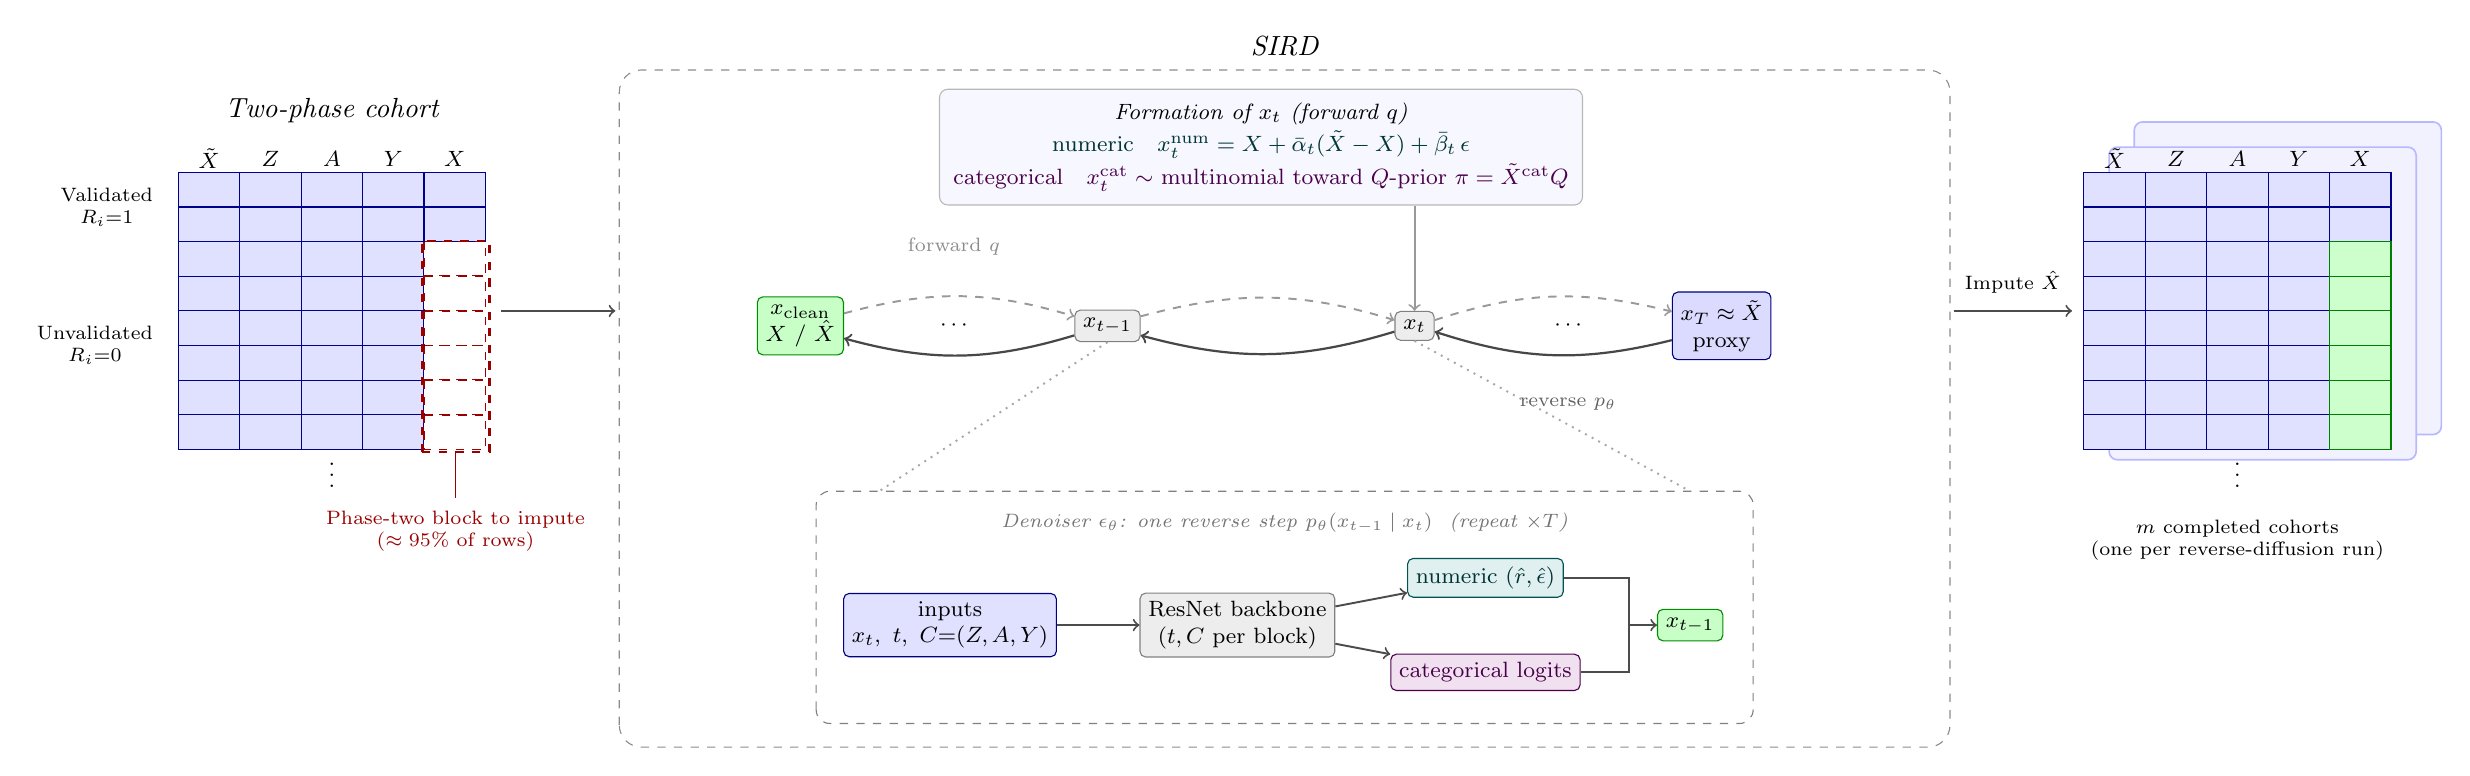
\begin{tikzpicture}[
  every node/.style={font=\footnotesize},
  obs/.style={fill=blue!12, draw=blue!55!black, line width=0.4pt},
  mis/.style={fill=white, draw=red!60!black, dashed, line width=0.6pt},
  imp/.style={fill=green!20, draw=green!50!black, line width=0.4pt},
  data/.style={rounded corners=2pt, draw=blue!50!black, fill=blue!12, align=center, inner sep=3pt},
  lyr/.style={rounded corners=2pt, draw=black!50, fill=black!7, align=center, inner sep=3pt},
  numbox/.style={rounded corners=2pt, draw=teal!65!black, fill=teal!12, align=center, inner sep=3pt, text=teal!40!black},
  catbox/.style={rounded corners=2pt, draw=violet!60!black, fill=violet!12, align=center, inner sep=3pt, text=violet!55!black},
  outbox/.style={rounded corners=2pt, draw=green!55!black, fill=green!22, align=center, inner sep=3pt},
  prx/.style={rounded corners=2pt, draw=blue!50!black, fill=blue!14, align=center, inner sep=3pt},
  formbox/.style={rounded corners=3pt, draw=black!28, fill=blue!3, align=center, inner sep=5pt},
  ghost/.style={rounded corners=3pt, fill=blue!5, draw=blue!28, line width=0.6pt},
  arr/.style={->, line width=0.7pt, draw=black!70},
  fwd/.style={->, line width=0.7pt, draw=black!40, dashed},
  rev/.style={->, line width=0.8pt, draw=black!72},
  callout/.style={dotted, draw=black!35, line width=0.7pt},
]
% ===== two-phase cohort (left) =====
\begin{scope}[shift={(1.4cm,10.0cm)}, x=0.78cm, y=0.44cm]
  \foreach \x/\lab in {0.5/{$\tilde{X}$}, 1.5/{$Z$}, 2.5/{$A$}, 3.5/{$Y$}, 4.5/{$X$}} \node at (\x,0.4) {\lab};
  \foreach \r in {0,1} \foreach \c in {0,1,2,3,4} \draw[obs] (\c,-\r) rectangle ++(1,-1);
  \foreach \r in {2,3,4,5,6,7} {
    \foreach \c in {0,1,2,3} \draw[obs] (\c,-\r) rectangle ++(1,-1);
    \draw[mis] (4,-\r) rectangle ++(1,-1);
  }
  \node at (2.5,-8.5) {$\vdots$};
\end{scope}
\node[font=\itshape] at (3.35,10.78) {Two-phase cohort};
\node[anchor=east, align=center, font=\scriptsize] at (1.2,9.56) {Validated\\$R_i{=}1$};
\node[anchor=east, align=center, font=\scriptsize] at (1.2,7.8) {Unvalidated\\$R_i{=}0$};
\draw[red!60!black, dashed, line width=0.9pt] (4.5,6.45) rectangle (5.35,9.13);
\draw[red!60!black, line width=0.6pt] (4.92,6.45) -- (4.92,5.86);
\node[anchor=north, align=center, font=\scriptsize, text=red!60!black] at (4.92,5.82) {Phase-two block to impute\\($\approx 95\%$ of rows)};
% ===== SIRD container =====
\draw[rounded corners=8pt, draw=black!45, dashed] (7.0,2.7) rectangle (23.9,11.3);
\node[font=\itshape] at (15.45,11.6) {SIRD};
% ===== diffusion chain =====
\node[outbox] (x0)  at (9.3,8.05)  {$x_{\mathrm{clean}}$\\ $X$ / $\hat X$};
\node[lyr]    (xtm) at (13.2,8.05) {$x_{t-1}$};
\node[lyr]    (xt)  at (17.1,8.05) {$x_t$};
\node[prx]    (xT)  at (21.0,8.05) {$x_T\approx\tilde X$\\ proxy};
\node at (11.25,8.05) {$\cdots$};
\node at (19.05,8.05) {$\cdots$};
\foreach \a/\b in {x0/xtm, xtm/xt, xt/xT}{
  \draw[fwd] (\a) to[bend left=16] (\b);
  \draw[rev] (\b) to[bend left=16] (\a);
}
\node[font=\scriptsize, text=black!45] at (11.25,9.05) {forward $q$};
\node[font=\scriptsize, text=black!62] at (19.05,7.05) {reverse $p_\theta$};
% ===== formation of x_t (above the chain) =====
\node[formbox] (form) at (15.15,10.32) {%
  {\itshape Formation of $x_t$ (forward $q$)}\\[2pt]
  \textcolor{teal!42!black}{numeric\quad $x_t^{\mathrm{num}}=X+\bar\alpha_t(\tilde X-X)+\bar\beta_t\,\epsilon$}\\[1pt]
  \textcolor{violet!58!black}{categorical\quad $x_t^{\mathrm{cat}}\sim$ multinomial toward $Q$-prior $\boldsymbol{\pi}=\tilde X^{\mathrm{cat}}Q$}};
\draw[->, draw=black!40, line width=0.7pt] (form.south -| xt) -- (xt.north);
% ===== denoiser zoom (one reverse step) =====
\draw[rounded corners=5pt, draw=black!50, dashed] (9.5,3.0) rectangle (21.4,5.95);
\node[font=\scriptsize\itshape, text=black!55] at (15.45,5.55) {Denoiser $\epsilon_\theta$: one reverse step $p_\theta(x_{t-1}\mid x_t)$ \ (repeat $\times T$)};
\node[data]   (zin)  at (11.2,4.25) {inputs\\ $x_t,\ t,\ C{=}(Z,A,Y)$};
\node[lyr]    (znet) at (14.85,4.25) {ResNet backbone\\ ($t,C$ per block)};
\node[numbox] (zhn)  at (18.0,4.85) {numeric $(\hat r,\hat\epsilon)$};
\node[catbox] (zhc)  at (18.0,3.65) {categorical logits};
\node[outbox] (zout) at (20.6,4.25) {$x_{t-1}$};
\draw[arr] (zin) -- (znet);
\draw[arr] (znet) -- (zhn);
\draw[arr] (znet) -- (zhc);
\coordinate (bus) at ([xshift=-3.5mm]zout.west);
\draw[line width=0.7pt, draw=black!70] (zhn.east) -| (bus);
\draw[line width=0.7pt, draw=black!70] (zhc.east) -| (bus);
\draw[arr] (bus) -- (zout.west);
\draw[callout] (xtm.south) -- (10.3,5.95);
\draw[callout] (xt.south)  -- (20.6,5.95);
% ===== cohort -> SIRD =====
\draw[arr] (5.5,8.24) -- (6.95,8.24);
% ===== m completed cohorts (right) =====
\draw[ghost] (26.24,6.67) rectangle (30.14,10.64);
\draw[ghost] (25.92,6.35) rectangle (29.82,10.32);
\begin{scope}[shift={(25.6cm,10.0cm)}, x=0.78cm, y=0.44cm]
  \foreach \x/\lab in {0.5/{$\tilde{X}$}, 1.5/{$Z$}, 2.5/{$A$}, 3.5/{$Y$}, 4.5/{$X$}} \node at (\x,0.4) {\lab};
  \foreach \r in {0,1} \foreach \c in {0,1,2,3,4} \draw[obs] (\c,-\r) rectangle ++(1,-1);
  \foreach \r in {2,3,4,5,6,7} {
    \foreach \c in {0,1,2,3} \draw[obs] (\c,-\r) rectangle ++(1,-1);
    \draw[imp] (4,-\r) rectangle ++(1,-1);
  }
  \node at (2.5,-8.5) {$\vdots$};
\end{scope}
\node[anchor=north, align=center, font=\scriptsize] at (27.55,5.71) {$m$ completed cohorts\\(one per reverse-diffusion run)};
\draw[arr] (23.95,8.24) -- (25.45,8.24);
\node[anchor=south, font=\scriptsize] at (24.7,8.34) {Impute $\hat X$};
\end{tikzpicture}%
}
\caption{SIRD with a fully observed outcome. The validated target block is missing outside phase two, while its proxies are observed for the full cohort. The continuous forward process moves the clean target toward its proxy, and the categorical process moves toward the paired transition prior. The reverse process uses the current state, time and remaining observed variables to return continuous residual and noise predictions and categorical logits. The displayed pipeline uses one fitted denoiser; the retained procedure repeats the fit on bootstrap samples. When outcome components also require validation, they enter the target block and their phase-one proxies remain observed.}
\label{fig:sird-architecture}
\end{sidewaysfigure}


\subsection{Reverse sampling and generating multiple imputations}
\label{sec:sird_mi}

Imputation runs the reverse chain for every individual with \(R_i=0\). The continuous state is initialised at the proxy endpoint,
\[
x_{T-1,i}=\tilde{X}_i+\sqrt{\eta}\,\xi_i,\qquad \xi_i\sim\mathcal{N}(0,I).
\]
For a paired categorical variable, the initial state is the mode of the proxy-induced distribution, \(\arg\max_k(\boldsymbol{\pi}_i)_k\); for an unpaired categorical variable it is a Gumbel-max draw from the uniform distribution. The chain then iterates \(t=T-1,\ldots,0\). At each step the network predicts the continuous residual and noise and forms
\[
\hat{x}_{\mathrm{clean},i}=x_{t,i}-\bar{\alpha}_t\hat I_{\mathrm{res},i}-\bar{\beta}_t\hat\epsilon_i.
\]
Write $A_t=\bar\alpha_t$, $V_t=\bar\beta_t^2$, $a_t=A_t-A_{t-1}$ and $v_t=V_t-V_{t-1}$, with $A_{-1}=V_{-1}=0$. For $t>0$, the continuous reverse mean and variance used by SIRD are
\begin{equation}
\begin{aligned}
\mu_t={}&\frac{V_{t-1}}{V_t}x_t
+\frac{v_tA_{t-1}-V_{t-1}a_t}{V_t}\hat I_{\mathrm{res}}
+\frac{v_t}{V_t}\hat x_{\mathrm{clean}},\\
\Sigma_t={}&\frac{v_tV_{t-1}}{V_t}I.
\end{aligned}
\label{eq:sird_cont_posterior}
\end{equation}
At $t=0$, the state is set to the predicted clean target. The categorical update uses equation~\eqref{eq:sird_cat_posterior}, with a Gumbel-max draw for $t>0$ and a deterministic $\arg\max$ at $t=0$. The final state is decoded to the original data scale.

With a single fitted denoiser, repeated reverse runs vary the diffusion noise but keep \(\theta\) fixed. The resulting \(m\) imputations therefore do not automatically propagate fitted-model uncertainty. The candidate mechanisms for adding that variation, MC-dropout, bootstrap retraining and SWAG, are evaluated in the ablation study of Section~\ref{sec:sird_uncertainty}. Algorithm~\ref{alg:sird} summarises the base single-fit procedure.

\begin{algorithm}[t]
\caption{Sample imputation via conditional residual denoising diffusion networks (SIRD): base fit and reverse sampler}
\label{alg:sird}
\begin{algorithmic}[1]
\Require Observed block $\{(\tilde X_i,C_i):i=1,\ldots,N\}$; validated targets $\{X_i:R_i=1\}$; imputations $m$; training steps $S_{\text{train}}$; diffusion steps $T$; residual schedule $\bar{\alpha}_t$; noise schedule $\bar{\beta}_t$; noise budget \(\eta\); loss weights $\lambda_{\text{num}}, \lambda_{\text{cat}}$
\Statex
\State Encode all variables (Section~\ref{sec:sird_encoding}); estimate transition matrices $Q$ via equation~\eqref{eq:transition_matrix}
\State Initialise denoiser $f_\theta$
\For{$s = 1, \ldots, S_{\text{train}}$} \Comment{Training (single fit)}
    \State Sample minibatch from $\{i : R_i = 1\}$
    \State $t \sim \mathrm{Unif}\{0, \ldots, T-1\}$; $\epsilon_i \sim \mathcal{N}(0,I)$
    \State Continuous: $x_{t,i} \gets X_i + \bar{\alpha}_t(\tilde{X}_i - X_i) + \bar{\beta}_t \epsilon_i$ \hfill (equation~\ref{eq:sird_cont_forward})
    \State Categorical: $x_{t,i} \sim \mathrm{Cat}\bigl((1-\bar{\alpha}_t) x_{\mathrm{clean},i} + \bar{\alpha}_t \boldsymbol{\pi}_i\bigr)$, $\boldsymbol{\pi}_i = (\tilde{x}_i^{\text{cat}})^\top Q$
    \State $(\hat{I}_{\text{res},i}, \hat{\epsilon}_i, \hat{x}_{\mathrm{clean},i}) \gets f_\theta(x_{t,i}, C_i, t)$
    \State Update $\theta$ by descending $\nabla_\theta(\mathcal{L}_{\text{num}} + \mathcal{L}_{\text{cat}})$ \hfill (equations~\ref{eq:sird_cont_loss},~\ref{eq:sird_cat_loss})
\EndFor
\Statex
\For{$j = 1, \ldots, m$} \Comment{Imputation: $m$ reverse runs, parameters $\theta$ fixed}
    \For{each $i$ with $R_i = 0$}
        \State Continuous init: $x_i \gets \tilde{X}_i + \sqrt{\eta}\, \xi$, $\xi \sim \mathcal{N}(0,I)$
        \State Categorical init: $x_i \gets \arg\max \boldsymbol{\pi}_i$ if paired, else a Gumbel-max draw with uniform class probabilities
        \For{$t = T-1, \ldots, 0$} \Comment{reverse chain}
            \State $(\hat{I}_{\text{res},i}, \hat{\epsilon}_i, \hat{x}_{\mathrm{clean},i}) \gets f_\theta(x_i, C_i, t)$
            \State Continuous: update from equation~\eqref{eq:sird_cont_posterior}
            \State Categorical: update from equation~\eqref{eq:sird_cat_posterior} ($\arg\max$ if $t=0$)
        \EndFor
        \State Inverse-transform the completed $x_i$ to the original scale; record as $X_i^{(j)}$
    \EndFor
\EndFor
\Ensure $m$ completed datasets $\{X_i^{(j)} : R_i = 0,\; j = 1, \ldots, m\}$
\end{algorithmic}
\end{algorithm}

The retained multiple-imputation procedure applies the following wrapper to the base fit. The encoding and transition priors are constructed once, while each completed dataset uses a denoiser fitted on a new bootstrap sample of the validated row indices.

\begin{algorithm}[t]
\caption{Sample imputation via conditional residual denoising diffusion networks (SIRD): retained bootstrap procedure}
\label{alg:sird_bootstrap}
\begin{algorithmic}[1]
\Require Encoded cohort and transition priors; validated index set $\mathcal V=\{i:R_i=1\}$; imputations $m$
\For{$j=1,\ldots,m$}
    \State Draw $\mathcal B_j$ by sampling $|\mathcal V|$ indices with replacement from $\mathcal V$
    \State Fit a new denoiser $f_{\theta_j}$ on $\mathcal B_j$ using the training stage of Algorithm~\ref{alg:sird}
    \State Run one reverse sampler with $f_{\theta_j}$ for all $i$ with $R_i=0$
    \State Store the resulting target block as completed dataset $j$
\EndFor
\Ensure $m$ completed datasets fitted from $m$ bootstrap samples
\end{algorithmic}
\end{algorithm}


\section{Ablation Study}
\label{sec:sird_ablation}

The SIRD configuration was selected by a staged ablation using the \texttt{SampleE}, \texttt{SRS} survival setting of Simulation Design~III, which was also used for the SICG ablation in Section~\ref{sec:sicg_ablation}. This ablation selects the components carried into the full comparison. The first stage compares the categorical state space while keeping the continuous residual construction fixed. The second tests classifier-free guidance on the retained residual--multinomial backbone. The third compares the mechanisms that create the \(m\) completed datasets and Rubin's between-imputation component \(B\). Table~\ref{tab:sird_ablation} reports the continuous, categorical and interaction results for these decisions. Table~\ref{tab:sird_bm} checks the amount of \(B\) supplied by the uncertainty mechanisms in the other analysis settings.

\begin{table}[!htbp]
\centering
\definecolor{rankone}{RGB}{33,113,181}\definecolor{ranktwo}{RGB}{107,174,214}\definecolor{rankthree}{RGB}{198,219,239}
\caption{Staged SIRD ablation on Simulation Design~III (\texttt{SampleE}, \texttt{SRS}, \(N=20{,}000\), \(n=1{,}000\), \(m=5\), \(500\) replicates). The coefficients are grouped into Continuous Phase-Two Covariates, Binary \& Categorical Phase-Two Covariates, and the age-by-insulin interaction. Each entry is the mean of the per-covariate metric within the block; Rel.\ RMSE is each coefficient's RMSE as a percentage of its true hazard ratio, averaged over the block. Columns are complete case (CC), naive proxy (UNVAL), single-fit residual--multinomial SIRD (MULT), Analog Bits categorical encoding (ANALOG), classifier-free guidance (CFG), bootstrap multiple imputation (BOOT, retained), MC-dropout (DROP), and SWAG. The three best distinct ranks among the non-CC/UNVAL methods are shaded; displayed ties receive the same shade. For Mean Bias rows, best means closest to zero. VAL is omitted because it defines the truth. The ablation fixes $m=5$ across all variants for comparability; the deployed SIRD configuration uses $m=20$ bootstrap imputations.}
\label{tab:sird_ablation}
\scriptsize
\setlength{\tabcolsep}{3.0pt}
\adjustbox{max width=\linewidth}{%
\begin{tabular}{lrrrrrrrr}
\toprule
 & \multicolumn{1}{c}{CC} & \multicolumn{1}{c}{UNVAL} & \multicolumn{1}{c}{MULT} & \multicolumn{1}{c}{ANALOG} & \multicolumn{1}{c}{CFG} & \multicolumn{1}{c}{\textbf{BOOT}} & \multicolumn{1}{c}{DROP} & \multicolumn{1}{c}{SWAG} \\
\midrule
\multicolumn{9}{l}{\textit{Continuous Phase-Two Covariates}} \\[2pt]
\quad Mean Bias (\%) & 0.3 & -0.3 & \cellcolor{rankone}-0.1 & \cellcolor{ranktwo}-0.2 & -0.4 & -0.5 & \cellcolor{rankthree}-0.3 & -0.4 \\
\quad Rel.\ RMSE (\%) & 5.2 & 8.0 & \cellcolor{ranktwo}2.1 & \cellcolor{rankthree}2.2 & \cellcolor{ranktwo}2.1 & \cellcolor{rankone}2.0 & 3.1 & 3.1 \\
\quad Nom.\ Cov. & 0.945 & 0.153 & \cellcolor{ranktwo}0.704 & 0.675 & \cellcolor{rankthree}0.677 & \cellcolor{rankone}0.840 & 0.431 & 0.442 \\
\quad Orc.\ Cov.\ (Emp) & 0.946 & 0.170 & \cellcolor{rankone}0.830 & \cellcolor{ranktwo}0.828 & \cellcolor{ranktwo}0.828 & \cellcolor{rankthree}0.766 & 0.634 & 0.569 \\
\quad Orc.\ Cov.\ (BC) & 0.949 & 0.913 & \cellcolor{rankthree}0.848 & 0.836 & 0.845 & \cellcolor{rankone}0.953 & 0.797 & \cellcolor{ranktwo}0.862 \\
\midrule
\multicolumn{9}{l}{\textit{Binary \& Categorical Phase-Two Covariates}} \\[2pt]
\quad Mean Bias (\%) & 4.9 & 6.3 & 5.4 & 5.9 & \cellcolor{ranktwo}4.6 & 5.1 & \cellcolor{rankone}4.0 & \cellcolor{rankthree}4.8 \\
\quad Rel.\ RMSE (\%) & 32.8 & 11.6 & \cellcolor{rankthree}10.2 & 10.5 & \cellcolor{rankone}9.6 & \cellcolor{ranktwo}9.7 & 10.3 & 10.4 \\
\quad Nom.\ Cov. & 0.969 & 0.585 & 0.923 & 0.750 & \cellcolor{ranktwo}0.936 & \cellcolor{rankthree}0.968 & 0.981 & \cellcolor{rankone}0.960 \\
\quad Orc.\ Cov.\ (Emp) & 0.944 & 0.622 & \cellcolor{ranktwo}0.829 & 0.794 & \cellcolor{rankone}0.840 & \cellcolor{rankthree}0.814 & 0.632 & 0.566 \\
\quad Orc.\ Cov.\ (BC) & 0.969 & 0.950 & \cellcolor{rankone}0.947 & \cellcolor{rankthree}0.922 & \cellcolor{ranktwo}0.946 & \cellcolor{rankthree}0.978 & 0.997 & 0.993 \\
\midrule
\multicolumn{9}{l}{\textit{Interaction}} \\[2pt]
\quad Mean Bias (\%) & 0.4 & 5.2 & -2.3 & \cellcolor{rankthree}-1.9 & -2.8 & -2.3 & \cellcolor{ranktwo}-1.3 & \cellcolor{rankone}-1.0 \\
\quad Rel.\ RMSE (\%) & 1.3 & 5.3 & 2.4 & \cellcolor{rankthree}2.0 & 2.8 & 2.4 & \cellcolor{ranktwo}1.4 & \cellcolor{rankone}1.2 \\
\quad Nom.\ Cov. & 0.938 & 0.000 & 0.036 & 0.058 & 0.008 & \cellcolor{rankthree}0.104 & \cellcolor{ranktwo}0.188 & \cellcolor{rankone}0.286 \\
\quad Orc.\ Cov.\ (Emp) & 0.944 & 0.000 & 0.062 & \cellcolor{rankthree}0.124 & 0.004 & 0.004 & \cellcolor{ranktwo}0.282 & \cellcolor{rankone}0.542 \\
\quad Orc.\ Cov.\ (BC) & 0.940 & 0.820 & 0.742 & 0.772 & 0.768 & \cellcolor{rankone}0.922 & \cellcolor{ranktwo}0.840 & \cellcolor{rankthree}0.802 \\
\bottomrule
\end{tabular}}
\end{table}

\subsection{Categorical state space}
\label{sec:sird_ablation_cat}

The categorical-stage comparison used the multinomial kernel of Section~\ref{sec:sird_multinomial} and the Analog Bits encoding of \citet{chen2023analog}. Analog Bits maps each category to a binary code, rescales the bits to \(\{-1,+1\}\), and diffuses the resulting bit vector in a continuous state space. This would keep the numeric and categorical blocks inside one Gaussian residual diffusion. The cost is that the proxy-to-truth transition matrix \(Q\) in equation~\eqref{eq:transition_matrix} no longer appears as the stationary distribution of a categorical forward process. In the ablation, this simplification was not accompanied by better Cox-model diagnostics. The continuous-block summaries were close to the multinomial row, while categorical nominal coverage was lower, \(0.750\) rather than \(0.923\). The decision is therefore local to the present SIRD construction: the multinomial kernel is retained because it matches the paired categorical information and performs better on the categorical block in this ablation.

\subsection{Conditioning guidance}
\label{sec:sird_ablation_guidance}

The next variant added classifier-free guidance (CFG) \citep{ho2022classifier}. During training, the conditioning vector \(C_i\) is randomly replaced by a learned null token. At sampling, conditional and unconditional predictions are combined with a guidance scale \(s>1\), which strengthens the effect of the conditioning information. Recent tabular diffusion work has assessed this device by distributional criteria \citep{shi2025tabdiff}; here it is assessed by downstream inference. Guidance changes continuous nominal coverage from \(0.704\) to \(0.677\) and interaction coverage from \(0.036\) to \(0.008\). Categorical coverage rises from \(0.923\) to \(0.936\), but the continuous and interaction results do not support retaining the guided variant.

\subsection{Uncertainty injection}
\label{sec:sird_uncertainty}

The final ablation stage compared MC-dropout, bootstrap retraining and SWAG on the retained residual--multinomial denoiser. The single-fit baseline produces \(m\) completed datasets by rerunning the reverse diffusion with fixed \(\hat\theta\); it therefore varies the reverse-sampling noise but not the fitted denoiser. Table~\ref{tab:sird_bm} reports the between-imputation variance \(B\) for the fitted coefficients involving the imputed continuous block, expressed as a multiple of this single-fit baseline. The table is a variance-injection diagnostic, not a coverage target.

\begin{table}[!htbp]
\centering
\caption{Between-imputation variance \(B\) for fitted coefficients involving the imputed continuous block, reported as a median multiple of the corresponding single-fit baseline. The Gaussian and Binomial rows each pool two fitted coefficients over 20 replicates per mechanism. The Cox row pools five continuous-block coefficients over 500 replicates per mechanism. The single-fit completed datasets differ only through reverse-sampling noise and define the baseline \(\equiv1\). These ratios compare variance injection within a row and are not targets for coverage.}
\label{tab:sird_bm}
\begin{tabular}{lrrr}
\toprule
Outcome model & Bootstrap & MC-dropout & SWAG \\
\midrule
Gaussian, Simulation Design~II & 214 & 16 & 3 \\
Binomial, Simulation Design~II & 147 & 2 & 4 \\
Cox, Simulation Design~III & 4 & 1 & 1 \\
\bottomrule
\end{tabular}
\end{table}

The bootstrap gives the largest median multiple in all three rows: \(214\) and \(147\) times the single-fit baseline in the Gaussian and Binomial models of Simulation Design~II, and \(4\) times in the Cox model of Simulation Design~III. MC-dropout is smaller, at \(16\), \(2\), and \(1\), while SWAG records \(3\), \(4\), and \(1\). These rows do not identify a single cause for the difference, because the settings differ in outcome model, coefficient scale, validation-sample size, number of imputed covariates entering the analysis, and link function. They do show the fact needed for the SIRD decision: on this diffusion backbone, MC-dropout gives little increase in the between-imputation variance of the fitted analysis coefficients in the Binomial and Cox rows, whereas the bootstrap gives the largest median \(B\) in all three rows.

On the continuous phase-two block in Table~\ref{tab:sird_ablation}, the single-fit multinomial baseline has nominal coverage \(0.704\) and bias-corrected oracle coverage \(0.848\). Bootstrap raises these to \(0.840\) and \(0.953\); MC-dropout and SWAG have nominal coverages of \(0.431\) and \(0.442\). The bootstrap is retained because it gives the largest median \(B\) in every row of Table~\ref{tab:sird_bm} and the highest observed continuous-block nominal and bias-corrected oracle coverage in the ablation. The retained procedure fits the proxy-referenced residual denoiser \(m\) times, which accounts for its higher runtime relative to SICG. Bootstrap spread adds fitted-model variation empirically and is not an exact posterior for neural-network weights \citep{bartlett2020bootstrap}. The age-by-insulin interaction remains poorly covered under the bootstrap, with nominal coverage \(0.104\) in the ablation, and is revisited below.

\section{Simulation Results}
\label{sec:sird_sim}

The ablation study fixes the SIRD configuration as the residual--multinomial denoiser with bootstrap multiple imputation. This section evaluates that configuration against the comparators of Section~\ref{sec:comparators} using the metrics of Section~\ref{sec:eval_metrics}. The aggregate tables average over model--design combinations. The design-specific interpretation retains all seven labels in Simulation Design~II and VCCC: \texttt{SRS}, \texttt{RS}, \texttt{WRS}, \texttt{SFS}, \texttt{ODS-Tail}, \texttt{Neyman-ODS} and \texttt{Neyman-IF}. Simulation Design~III retains \texttt{SRS}, \texttt{Balanced} and \texttt{Neyman-IF} under both \texttt{SampleE} and \texttt{SampleOE}. Tables~\ref{tab:sird_rank_nutri} to~\ref{tab:sird_rank_vccc} give the aggregate summaries. Tables~\ref{tab:appc_nutri_Gaussian} to~\ref{tab:appc_vccc_COX} and Figures~\ref{fig:appc_simI_focal} to~\ref{fig:appc_vccc_cox} give the design-specific results.

SIRD imputes the phase-two block jointly, but the downstream terms differ in bias and coverage. The results are therefore reported separately for the continuous block, the categorical block and the interaction where it is present, using the same groups as Chapter~\ref{chap:SICG}.

The aggregate evidence for SIRD is strongest on the continuous phase-two covariates. Its log-scale mean absolute bias is \(3.5\%\) in Simulation Design~II, \(1.3\%\) in Simulation Design~III and \(2.9\%\) in VCCC; the corresponding SICG values are \(10.7\%\), \(1.5\%\) and \(3.9\%\). SIRD also reduces SICG's relative RMSE from \(18.1\%\) to \(11.0\%\) in Design~II and from \(2.9\%\) to \(2.5\%\) in Design~III. Nominal coverage is \(0.93\) and \(0.89\), compared with \(0.26\) and \(0.62\) for SICG. The first value is close to nominal; the second remains below \(0.95\). Table~\ref{tab:sird_bm} separately shows that bootstrap produces the largest median \(B\) among the tested SIRD uncertainty procedures within each row.

The categorical block also gives a positive result. In Simulation Design~III, SIRD has mean absolute bias \(2.1\%\), relative RMSE \(11.1\%\), nominal coverage \(0.99\), and an SE ratio of \(1.40\). The intervals are conservative on average. The random-forest and boosted-tree procedures have lower relative RMSE, at \(6.8\%\) and \(8.8\%\), and \texttt{mixgb} has comparable bias at \(2.0\%\). SIRD therefore improves on SICG for this block without becoming the most precise categorical method. In Design~II, SIRD has the smallest aggregate mean absolute interaction bias among the imputation methods, \(21.4\%\), with nominal coverage \(0.94\). In Design~III, the interaction bias falls from SICG's \(6.5\%\) to \(3.5\%\), while nominal coverage remains \(0.03\). The product-term result is compatible with imputation-analysis mismatch \citep{meng1994multiple}, but the experiment does not identify its cause.

\subsection{Simulation Design II}
\label{sec:sird_sim_nutri}

Simulation Design~II requires the most explicit design-level reading. Tables~\ref{tab:appc_nutri_Gaussian} and~\ref{tab:appc_nutri_Binomial} first show the three probability designs. \texttt{SRS} uses a common sampling fraction, and \texttt{Neyman-ODS} is close to proportional allocation. \texttt{Neyman-IF} allocates more validation to the two outer outcome strata, where the approximate influence function has greater spread. In all three rows, raking's exposure bias is close to zero and its nominal coverage is near \(0.95\) in both outcome models. SIRD is farther from the full-data exposure coefficient, although its nominal coverage is also close to the target: \(0.94\), \(0.94\) and \(0.95\) in the Gaussian model, and \(0.94\), \(0.93\) and \(0.92\) in the Binomial model.

The \texttt{RS}, \texttt{WRS}, \texttt{SFS} and \texttt{ODS-Tail} rows have a different structure. They concentrate validation in residual, weighted-residual, score-function or outcome tails, following the validation-design strategies studied by \citet{amorim2021two}. For SIRD, these rows also differ in the information passed to the denoiser: the proxy \(\tilde X_i\) anchors the residual endpoint, \(Y_i\) enters the conditioning vector \(C_i\), and the \texttt{RS}, \texttt{WRS} and \texttt{SFS} datasets include the corresponding residual, weighted-residual or score variable as an auxiliary input. The denoiser conditions on these variables rather than estimating the sampling rule. In the Gaussian model, raking's nominal coverage is \(0.00\), \(0.00\), \(0.00\) and \(0.01\) under these four rows, while the corresponding SIRD coverages are \(0.80\), \(0.98\), \(0.98\) and \(0.89\). The associated exposure biases are also smaller for SIRD in these rows: \(7.6\%\), \(1.3\%\), \(0.4\%\) and \(5.2\%\), compared with \(64.7\%\), \(64.0\%\), \(63.8\%\) and \(30.4\%\) for raking. In the Binomial model, the same four rows give raking coverages \(0.18\), \(0.10\), \(0.07\) and \(0.35\), compared with \(0.94\), \(0.94\), \(0.92\) and \(0.93\) for SIRD. Because the aggregate table averages rows with different validation rules, it cannot support a general ranking of SIRD over raking. In the non-tail rows raking remains the lower-bias reference; in the tail-enrichment rows Appendix~\ref{app:supp_fullsim} shows large exposure-coefficient displacement for raking and several other methods, while SIRD is less displaced on the reported exposure coefficient and has higher nominal coverage in those rows.

For the exposure-by-age interaction, SIRD has the smallest aggregate mean absolute bias among the imputation methods, \(21.4\%\), and the highest nominal coverage, \(0.94\). Its empirical oracle coverage is \(0.91\), and its bias-corrected oracle coverage is \(0.97\). TabCSDI and \texttt{mice.impute.rf} have lower relative RMSE of the coefficient estimate, so SIRD leads the bias and coverage comparisons but not RMSE. Figure~\ref{fig:appc_simI_focal} gives the same reading without aggregation: in several \texttt{RS}, \texttt{WRS}, \texttt{SFS} and \texttt{ODS-Tail} panels, the SIRD distributions are closer to zero than the SICG distributions, while the \texttt{SRS}, \texttt{Neyman-ODS} and \texttt{Neyman-IF} panels still indicate raking as the lower-bias reference.

\begin{table}[!htbp]\centering
\definecolor{rankone}{RGB}{33,113,181}\definecolor{ranktwo}{RGB}{107,174,214}\definecolor{rankthree}{RGB}{198,219,239}
\caption{Method performance on the focal coefficients of Simulation Design~II, summarised over its 14 model$\times$design combinations. Mean $|$bias$|$ and relative RMSE are averaged across coefficients and combinations on the log scale. This reduces the influence of extreme relative errors when a true coefficient is close to zero, although relative metrics still require caution near the null. Coverages are ordinary arithmetic means against the nominal $0.95$. The three best distinct ranks per row, including the complete-case and naive-proxy references, are shaded; displayed ties receive the same shade.}
\label{tab:sird_rank_nutri}
\scriptsize
\setlength{\tabcolsep}{3.5pt}
\adjustbox{max width=\linewidth}{%
\begin{tabular}{lrrrrrrrrrr}
\toprule
 & \multicolumn{1}{c}{CC} & \multicolumn{1}{c}{UNVAL} & \multicolumn{1}{c}{MICE-PMM} & \multicolumn{1}{c}{MICE-RF} & \multicolumn{1}{c}{MIXGB} & \multicolumn{1}{c}{TabCSDI} & \multicolumn{1}{c}{GAIN} & \multicolumn{1}{c}{RAKING} & \multicolumn{1}{c}{\textbf{SICG}} & \multicolumn{1}{c}{\textbf{SIRD}} \\
\midrule
\multicolumn{11}{l}{\textit{Continuous Phase-Two Covariates}} \\[2pt]
\quad Mean $|$Bias$|$ (\%) & \cellcolor{ranktwo}5.9 & 63.6 & 41.4 & 46.1 & 42.2 & 13.3 & 54.9 & \cellcolor{rankthree}7.1 & 10.7 & \cellcolor{rankone}3.5 \\
\quad Rel.\ RMSE (\%) & 26.6 & 63.7 & 43.5 & 46.4 & 50.2 & \cellcolor{rankthree}23.4 & 102.0 & 30.7 & \cellcolor{ranktwo}18.1 & \cellcolor{rankone}11.0 \\
\quad SE ratio & \cellcolor{ranktwo}1.03 & \cellcolor{rankone}1.01 & 0.39 & 0.62 & 0.74 & 0.24 & 0.04 & 0.78 & 0.32 & \cellcolor{rankthree}1.13 \\
\quad Nom.\ Cov. & \cellcolor{ranktwo}0.64 & 0.00 & 0.07 & 0.00 & 0.41 & 0.10 & 0.07 & \cellcolor{rankthree}0.45 & 0.26 & \cellcolor{rankone}0.93 \\
\quad Orc.\ Cov.\ (Emp) & \cellcolor{ranktwo}0.64 & 0.00 & 0.11 & 0.00 & 0.44 & 0.40 & \cellcolor{rankone}0.90 & \cellcolor{rankthree}0.51 & \cellcolor{ranktwo}0.64 & \cellcolor{rankone}0.90 \\
\quad Orc.\ Cov.\ (BC) & \cellcolor{rankone}0.95 & \cellcolor{ranktwo}0.96 & 0.77 & 0.86 & 0.79 & 0.58 & 0.07 & \cellcolor{rankthree}0.87 & 0.49 & \cellcolor{rankone}0.95 \\
\midrule
\multicolumn{11}{l}{\textit{Interaction}} \\[2pt]
\quad Mean $|$Bias$|$ (\%) & \cellcolor{ranktwo}22.1 & 64.8 & 345.3 & 56.4 & 48.1 & 39.8 & 116.9 & 42.4 & \cellcolor{rankthree}38.3 & \cellcolor{rankone}21.4 \\
\quad Rel.\ RMSE (\%) & 193.6 & \cellcolor{rankthree}89.6 & 360.7 & \cellcolor{ranktwo}76.7 & 146.9 & \cellcolor{rankone}70.1 & 297.4 & 224.8 & 115.9 & 93.6 \\
\quad SE ratio & \cellcolor{ranktwo}1.07 & \cellcolor{ranktwo}0.93 & \cellcolor{ranktwo}0.93 & 1.36 & 0.73 & \cellcolor{rankone}1.06 & 0.23 & \cellcolor{rankthree}0.88 & 0.53 & 1.15 \\
\quad Nom.\ Cov. & \cellcolor{ranktwo}0.93 & 0.47 & 0.09 & 0.63 & 0.75 & 0.69 & 0.38 & \cellcolor{rankthree}0.79 & 0.60 & \cellcolor{rankone}0.94 \\
\quad Orc.\ Cov.\ (Emp) & \cellcolor{ranktwo}0.90 & 0.47 & 0.12 & 0.52 & 0.83 & 0.66 & 0.81 & \cellcolor{rankthree}0.89 & 0.83 & \cellcolor{rankone}0.91 \\
\quad Orc.\ Cov.\ (BC) & \cellcolor{ranktwo}0.96 & \cellcolor{rankone}0.95 & 0.92 & 0.99 & 0.87 & \cellcolor{rankthree}0.97 & 0.51 & 0.89 & 0.77 & \cellcolor{rankthree}0.97 \\
\bottomrule
\end{tabular}}
\end{table}

\subsection{Simulation Design III}
\label{sec:sird_sim_surv}

Simulation Design~III uses \texttt{SRS}, \texttt{Balanced} and \texttt{Neyman-IF} under both \texttt{SampleE} and \texttt{SampleOE}; it excludes the tail-enrichment rows of Simulation Design~II. Raking has aggregate mean absolute bias \(0.1\%\) and nominal coverage \(0.92\) on the continuous block. SIRD has mean absolute bias \(1.3\%\), relative RMSE \(2.5\%\), nominal coverage \(0.89\), and an SE ratio of \(1.37\). SICG records \(1.5\%\), \(2.9\%\), \(0.62\), and \(0.59\). SIRD therefore improves on SICG, although its coverage remains below nominal and its reported standard errors exceed the empirical spread on average. Bias-corrected oracle coverage of \(0.98\) indicates that average displacement contributes to the remaining coverage pattern; it does not establish standard-error calibration.

On the categorical block, SIRD has mean absolute bias \(2.1\%\), relative RMSE \(11.1\%\), nominal coverage \(0.99\), and an SE ratio of \(1.40\). The tree procedures retain the lower RMSE. This block is not governed by the residual trajectory that drives the continuous result: its correction depends on the proxy-to-truth transition prior and on the denoiser's ability to use the less frequent off-diagonal transitions rather than simply preserving the phase-one category. The categorical component therefore has low bias and conservative coverage, while working through a weaker mechanism than the continuous path.

The age-by-insulin interaction is the exception. SIRD reduces the log-scale mean absolute interaction bias of SICG from \(6.5\%\) to \(3.5\%\), but nominal coverage remains \(0.03\). The empirical-standard-error oracle is also near zero, while the bias-corrected oracle is \(0.99\). Replacing the reported standard errors by the empirical standard error does not restore coverage because the remaining bias is large relative to the standard errors. The result is compatible with an imputation-analysis mismatch for the product term, but the experiment does not distinguish that explanation from other features of the survival setting. Figures~\ref{fig:appc_simII_cont} to~\ref{fig:appc_simII_inter} show the separation visually: the continuous and categorical coefficient blocks behave differently from the interaction.

\begin{table}[!htbp]\centering
\definecolor{rankone}{RGB}{33,113,181}\definecolor{ranktwo}{RGB}{107,174,214}\definecolor{rankthree}{RGB}{198,219,239}
\caption{Method performance on the focal coefficients of Simulation Design~III, summarised over its 6 model$\times$design combinations. Mean $|$bias$|$ and relative RMSE are averaged across coefficients and combinations on the log scale. This reduces the influence of extreme relative errors when a true coefficient is close to zero, although relative metrics still require caution near the null. Coverages are ordinary arithmetic means against the nominal $0.95$. The three best distinct ranks per row, including the complete-case and naive-proxy references, are shaded; displayed ties receive the same shade. TabCSDI was not run in this design because of its computational cost.}
\label{tab:sird_rank_surv}
\scriptsize
\setlength{\tabcolsep}{3.5pt}
\adjustbox{max width=\linewidth}{%
\begin{tabular}{lrrrrrrrrrr}
\toprule
 & \multicolumn{1}{c}{CC} & \multicolumn{1}{c}{UNVAL} & \multicolumn{1}{c}{MICE-PMM} & \multicolumn{1}{c}{MICE-RF} & \multicolumn{1}{c}{MIXGB} & \multicolumn{1}{c}{TabCSDI} & \multicolumn{1}{c}{GAIN} & \multicolumn{1}{c}{RAKING} & \multicolumn{1}{c}{\textbf{SICG}} & \multicolumn{1}{c}{\textbf{SIRD}} \\
\midrule
\multicolumn{11}{l}{\textit{Continuous Phase-Two Covariates}} \\[2pt]
\quad Mean $|$Bias$|$ (\%) & \cellcolor{ranktwo}1.2 & 6.0 & 3.8 & 4.5 & 2.0 & -- & 2.9 & \cellcolor{rankone}0.1 & 1.5 & \cellcolor{rankthree}1.3 \\
\quad Rel.\ RMSE (\%) & 4.4 & 6.3 & 5.1 & 4.6 & \cellcolor{rankthree}3.1 & -- & 14.0 & 3.5 & \cellcolor{ranktwo}2.9 & \cellcolor{rankone}2.5 \\
\quad SE ratio & \cellcolor{rankone}1.00 & \cellcolor{rankthree}0.91 & 1.16 & 1.78 & 0.78 & -- & 0.10 & \cellcolor{ranktwo}0.93 & 0.59 & 1.37 \\
\quad Nom.\ Cov. & \cellcolor{rankthree}0.79 & 0.14 & 0.61 & 0.13 & 0.44 & -- & 0.15 & \cellcolor{rankone}0.92 & 0.62 & \cellcolor{ranktwo}0.89 \\
\quad Orc.\ Cov.\ (Emp) & 0.79 & 0.15 & 0.52 & 0.05 & 0.54 & -- & \cellcolor{ranktwo}0.89 & \cellcolor{rankone}0.95 & \cellcolor{rankthree}0.80 & 0.76 \\
\quad Orc.\ Cov.\ (BC) & \cellcolor{rankone}0.95 & 0.91 & \cellcolor{ranktwo}0.93 & 0.99 & 0.87 & -- & 0.17 & \cellcolor{rankthree}0.92 & 0.78 & \cellcolor{rankthree}0.98 \\
\midrule
\multicolumn{11}{l}{\textit{Binary \& Categorical Phase-Two Covariates}} \\[2pt]
\quad Mean $|$Bias$|$ (\%) & 3.0 & 6.2 & 13.4 & \cellcolor{rankthree}2.5 & \cellcolor{rankone}2.0 & -- & 6.5 & 2.6 & 3.5 & \cellcolor{ranktwo}2.1 \\
\quad Rel.\ RMSE (\%) & 23.3 & \cellcolor{rankthree}9.0 & 22.9 & \cellcolor{rankone}6.8 & \cellcolor{ranktwo}8.8 & -- & 39.2 & 24.9 & 13.5 & 11.1 \\
\quad SE ratio & \cellcolor{ranktwo}1.01 & \cellcolor{rankone}1.00 & 0.90 & 1.96 & \cellcolor{rankthree}0.93 & -- & 0.23 & \cellcolor{rankthree}0.93 & 0.72 & 1.40 \\
\quad Nom.\ Cov. & \cellcolor{rankone}0.95 & 0.56 & 0.67 & 1.00 & \cellcolor{rankthree}0.92 & -- & 0.35 & \cellcolor{ranktwo}0.93 & 0.83 & 0.99 \\
\quad Orc.\ Cov.\ (Emp) & \cellcolor{ranktwo}0.94 & 0.59 & 0.74 & 0.84 & \cellcolor{rankthree}0.93 & -- & \cellcolor{rankone}0.95 & \cellcolor{rankone}0.95 & \cellcolor{rankthree}0.93 & 0.90 \\
\quad Orc.\ Cov.\ (BC) & \cellcolor{ranktwo}0.96 & \cellcolor{rankone}0.95 & 0.90 & 1.00 & \cellcolor{rankthree}0.93 & -- & 0.37 & \cellcolor{rankthree}0.93 & 0.84 & 0.99 \\
\midrule
\multicolumn{11}{l}{\textit{Interaction}} \\[2pt]
\quad Mean $|$Bias$|$ (\%) & \cellcolor{ranktwo}0.4 & 4.3 & 5.1 & 7.0 & \cellcolor{rankthree}3.4 & -- & 5.6 & \cellcolor{rankone}0.1 & 6.5 & 3.5 \\
\quad Rel.\ RMSE (\%) & \cellcolor{ranktwo}1.1 & 4.4 & 5.1 & 7.0 & \cellcolor{rankthree}3.4 & -- & 6.3 & \cellcolor{rankone}1.0 & 6.5 & 3.5 \\
\quad SE ratio & \cellcolor{rankone}1.00 & 0.57 & \cellcolor{rankone}1.00 & 2.50 & \cellcolor{rankthree}0.67 & -- & 0.19 & \cellcolor{ranktwo}0.80 & 1.67 & 1.50 \\
\quad Nom.\ Cov. & \cellcolor{ranktwo}0.86 & 0.00 & 0.00 & 0.00 & 0.01 & -- & \cellcolor{rankthree}0.08 & \cellcolor{rankone}0.90 & 0.00 & 0.03 \\
\quad Orc.\ Cov.\ (Emp) & \cellcolor{ranktwo}0.88 & 0.00 & 0.00 & 0.00 & 0.01 & -- & \cellcolor{rankthree}0.27 & \cellcolor{rankone}0.95 & 0.00 & 0.00 \\
\quad Orc.\ Cov.\ (BC) & \cellcolor{rankone}0.94 & 0.82 & \cellcolor{rankone}0.94 & \cellcolor{rankthree}1.00 & 0.82 & -- & 0.27 & \cellcolor{ranktwo}0.91 & \cellcolor{ranktwo}0.99 & \cellcolor{ranktwo}0.99 \\
\bottomrule
\end{tabular}}
\end{table}

\subsection{The VCCC case study}
\label{sec:sird_sim_vccc}

The VCCC case study is used as an applied check. On the focal Phase-Two covariates, raking has the smallest log-scale mean absolute bias, \(1.7\%\), with SIRD at \(2.9\%\) and SICG at \(3.9\%\); the relative RMSE of the coefficient estimate is similar across the three rows and slightly favours SIRD, \(7.0\%\), \(6.1\%\) and \(7.1\%\) for raking, SIRD and SICG. For nominal coverage, SIRD records \(0.99\), compared with \(0.95\) for raking and \(0.96\) for SICG. The oracle pattern is different from the two simulations. Raking has empirical-standard-error oracle coverage \(0.51\), SICG has \(0.60\), and SIRD has \(0.66\), while the corresponding bias-corrected oracle coverages are \(0.99\), \(0.97\) and \(0.99\). The low empirical-standard-error oracle coverage occurs for all three methods and is treated as a shared case-study pattern under repeated validation subsampling against a fixed full-data target, rather than as evidence about the SIRD uncertainty mechanism.

The detailed VCCC tables, Tables~\ref{tab:appc_vccc_LM} to~\ref{tab:appc_vccc_COX}, give the same compact reading. Several rows already have small bias for multiple methods, and the aggregate summary is not used to rank uncertainty mechanisms. The case study is therefore supportive evidence for applied coefficient-estimate behaviour; the uncertainty mechanism is assessed in the two simulation settings.

\begin{table}[!htbp]\centering
\definecolor{rankone}{RGB}{33,113,181}\definecolor{ranktwo}{RGB}{107,174,214}\definecolor{rankthree}{RGB}{198,219,239}
\caption{Method performance on the focal coefficients of the VCCC case study, summarised over its 21 model$\times$design combinations. Mean $|$bias$|$ and relative RMSE are averaged across coefficients and combinations on the log scale. This reduces the influence of extreme relative errors when a true coefficient is close to zero, although relative metrics still require caution near the null. Coverages are ordinary arithmetic means against the nominal $0.95$. The three best distinct ranks per row, including the complete-case and naive-proxy references, are shaded; displayed ties receive the same shade. The naive-proxy estimate is computed once on the fixed cohort, so its empirical standard error and related entries are unavailable.}
\label{tab:sird_rank_vccc}
\scriptsize
\setlength{\tabcolsep}{3.5pt}
\adjustbox{max width=\linewidth}{%
\begin{tabular}{lrrrrrrrrrr}
\toprule
 & \multicolumn{1}{c}{CC} & \multicolumn{1}{c}{UNVAL} & \multicolumn{1}{c}{MICE-PMM} & \multicolumn{1}{c}{MICE-RF} & \multicolumn{1}{c}{MIXGB} & \multicolumn{1}{c}{TabCSDI} & \multicolumn{1}{c}{GAIN} & \multicolumn{1}{c}{RAKING} & \multicolumn{1}{c}{\textbf{SICG}} & \multicolumn{1}{c}{\textbf{SIRD}} \\
\midrule
\multicolumn{11}{l}{\textit{Continuous Phase-Two Covariates}} \\[2pt]
\quad Mean $|$Bias$|$ (\%) & 6.2 & 7.6 & 13.0 & 9.7 & 22.2 & 11.0 & 7.4 & \cellcolor{rankone}1.7 & \cellcolor{rankthree}3.9 & \cellcolor{ranktwo}2.9 \\
\quad Rel.\ RMSE (\%) & 19.1 & 7.6 & 18.9 & 12.9 & 24.4 & 14.9 & 19.8 & \cellcolor{ranktwo}7.0 & \cellcolor{rankthree}7.1 & \cellcolor{rankone}6.1 \\
\quad SE ratio & 2.80 & -- & \cellcolor{rankthree}2.08 & 3.00 & 2.18 & \cellcolor{rankone}1.06 & \cellcolor{ranktwo}0.53 & 4.25 & 2.12 & 2.75 \\
\quad Nom.\ Cov. & 0.84 & 0.71 & 0.58 & 0.85 & 0.69 & 0.56 & 0.62 & \cellcolor{rankone}0.95 & \cellcolor{ranktwo}0.96 & \cellcolor{rankthree}0.99 \\
\quad Orc.\ Cov.\ (Emp) & 0.48 & -- & 0.35 & 0.30 & 0.22 & 0.47 & \cellcolor{rankone}0.91 & 0.51 & \cellcolor{rankthree}0.60 & \cellcolor{ranktwo}0.66 \\
\quad Orc.\ Cov.\ (BC) & 0.99 & 1.00 & \cellcolor{rankthree}0.98 & 1.00 & 1.00 & \cellcolor{rankone}0.95 & 0.72 & 0.99 & \cellcolor{ranktwo}0.97 & 0.99 \\
\bottomrule
\end{tabular}}
\end{table}


\section{Discussion}
\label{sec:sird_discussion}

This chapter took up the problem Chapter~\ref{chap:SICG} left open. The obstacle identified there was specific: the barrier to valid two-phase inference with a generative imputer lay in carrying fitted-model uncertainty into the between-imputation variance, not in the accuracy of the coefficient estimate, and the cost of an adversarial fit made the natural remedy, repeated refitting, infeasible. SIRD answers that problem by using the phase-one proxy as the reference endpoint of its generative path. For a paired continuous variable, the denoiser learns the measurement-error residual \(\tilde X_i-X_i\) around that reference \citep{liu2024residual,ho2020denoising,kotelnikov2023tabddpm}. The retained proxy-referenced, non-adversarial denoiser is fitted separately for 20 bootstrap imputations. Those fits explain its longer runtime than SICG. The full procedure gives lower coefficient bias and coverage closer to \(0.95\) than SICG on the continuous block, together with useful categorical estimates. The Cox interaction remains poorly covered.

On the continuous phase-two block, aggregate nominal coverage is \(0.93\) in Simulation Design~II and \(0.89\) in Simulation Design~III, against \(0.26\) and \(0.62\) for SICG. The corresponding mean absolute biases are \(3.5\%\) and \(1.3\%\). In the Gaussian model of Design~II, SIRD coverage is \(0.94\) under \texttt{SRS} and ranges from \(0.80\) to \(0.98\) across the four tail-enrichment designs. Its Binomial coverage ranges from \(0.92\) to \(0.94\) across all seven designs. Raking retains lower exposure bias in the non-tail rows and throughout Design~III. In the tail rows, SIRD is fitted with the selection variable or the phase-one information used to form it and records lower bias and higher coverage. These comparisons show its performance when that information is supplied; they do not estimate the separate effect of adding it or show that SIRD recovers the sampling rule.

The continuous-block SE ratio is \(1.13\) in Design~II and \(1.37\) in Design~III, compared with \(0.32\) and \(0.59\) for SICG. SIRD's reported standard errors are close to the empirical spread in Design~II and conservative on average in Design~III. The bootstrap fits add fitted-model variation, while the coefficient-estimate improvement belongs to the full SIRD construction. The Cox age-by-insulin interaction separates the two properties: its SE ratio is \(1.50\), so its reported standard error is conservative relative to the empirical spread, while nominal coverage is only \(0.03\). Together with bias-corrected oracle coverage of \(0.99\), this pattern points to displacement of the estimate rather than a reported variance that is too small.

Table~\ref{tab:sird_bm} has a narrower use. Within each row, bootstrap gives the largest median \(B\): about \(214\) and \(147\) times the single-fit baseline in the Gaussian and Binomial models, and about \(4\) times it in the Cox model. Ratios cannot be compared as absolute uncertainty measures across these settings or with the SICG table because the coefficient scales, validation-sample sizes, analysis models and single-fit baselines differ. The Cox ratio does not show that a single fit is adequately dispersed or that fewer refits would suffice. The table supports the choice among the tested SIRD procedures and no stronger conclusion.

Design~III gives a positive categorical result. SIRD has mean absolute bias \(2.1\%\), relative RMSE \(11.1\%\), nominal coverage \(0.99\), and an SE ratio of \(1.40\). The coefficient estimates improve on SICG and the intervals are conservative on average. Random forest and \texttt{mixgb} remain more precise, with relative RMSE of \(6.8\%\) and \(8.8\%\). The categorical component therefore works well in location and coverage, although it does not lead the precision comparison.

The interaction results differ by analysis. Across the Gaussian and Binomial models of Design~II, aggregate nominal coverage is \(0.94\), empirical-standard-error oracle coverage is \(0.91\), and bias-corrected oracle coverage is \(0.97\). Mean absolute relative bias remains \(21.4\%\), and relative RMSE is \(93.6\%\): the intervals cover because the term is estimated imprecisely and its standard error is large relative to the small effect, not because the estimate is centred. In the Cox model of Design~III, nominal coverage ranges from \(0.00\) to \(0.09\), the empirical-standard-error oracle remains near zero, and the bias-corrected oracle ranges from \(0.96\) to \(1.00\). The oracle substitutions point to average displacement of the product-term estimate. Several imputation methods share this problem, while raking remains close to nominal. That pattern points to uncongeniality \citep{meng1994multiple}: the completed data do not preserve the insulin-by-age relationship the analysis uses, and the failure is shared across imputation architectures rather than produced by the hazard model, which raking fits without failing.

Simulation Design~I provides a separate displacement result. SIRD does not use the released design weight in that privacy-constrained setting. Its exposure bias is \(19.8\%\), SE ratio is \(1.50\), empirical-standard-error oracle coverage is \(0.21\), and bias-corrected oracle coverage is \(0.98\). The reported standard error is conservative relative to the empirical spread, while the oracle pattern points to average displacement from the informative selection. Chapter~\ref{chap:SISL} reports the methods designed to use the released weight.

VCCC is used as an applied coefficient-estimate check. SIRD has focal continuous bias of \(2.9\%\), compared with \(3.9\%\) for SICG, and nominal coverage of \(0.99\). Its empirical-standard-error oracle coverage is \(0.66\), within a case-study pattern also seen for raking and SICG, so VCCC is not used to assess repeated-sampling calibration. SIRD still depends on an informative paired proxy, and the retained bootstrap requires 20 denoiser fits. The latter cost is intentional: each completed dataset is tied to a separate bootstrap refit, rather than to another reverse run from one fitted network.

The main contribution is the use of the phase-one proxy inside the diffusion path. For continuous variables, the proxy defines an informative endpoint and the network learns \(\tilde X_i-X_i\). For categorical variables, the paired data define the transition prior. The complete SIRD procedure gives better coefficient estimates and interval coverage than SICG across both blocks. Bootstrap refitting supplies fitted-model variation for the intervals; the ablation does not identify it as the source of the coefficient-estimate improvement. Design~III coverage is conservative and remains below nominal on the continuous block. Raking remains the lower-bias reference where its calibration equations apply. More generally, the results imply that a generative imputation model should be judged by the coefficient estimate and the total variance \(T=\bar U+(1+1/m)B\) it produces, and by whether the completed data preserve the features of the analysis on which the inference depends, such as the relevant cross-moments, rather than by distributional-fidelity metrics alone.

Future work should address the Cox-model product term directly and should evaluate any cheaper uncertainty procedure by repeated-sampling coverage, rather than infer its adequacy from a small \(B\) multiple. An analysis-aware objective that preserves the relevant covariate cross-moment is one testable option. The present results do not establish that such an objective will remove the displacement.
